\section{选择操作}

\subsection{基本算法}

文件扫描---定位并检索满足选择条件的记录的搜索算法,不使用索引。

\noindent算法A1(线性搜索):扫描每个文件块并测试所有记录,查看它们是否满足选择条件。
\begin{itemize}
    \item 成本估算$=b_r$块传输+1寻道:$b_r$表示包含来自关系$r$的记录的块数
    \item 如果选择是基于键属性,则在找到记录时可以停止:成本$=(b_r/2)$块传输+1寻道
    \item 线性搜索无论:选择条件、文件中记录的排序、索引的可用性
\end{itemize}

注意:由于数据并非连续存储,二分查找通常没有意义。除非有可用的索引,并且二分查找比索引查找需要更多的查找操作。

\noindent算法A2(二分查找):若选择操作是对文件排序所依据的属性进行相等比较,则适用。
\begin{itemize}
    \item 假设关系的块是连续存储的
    \item 成本$=\lceil \log_2(b_r) \rceil$块传输$+\lceil \log_2(b_r) \rceil$通过对块进行二分查找来定位第一个元组的寻道成本(时间成本$=\lceil \log_2(b_r) \rceil*(t_S+t_T)$)
    \item 如果选择操作不是针对键属性,则需要加上包含满足选择条件记录的块的数量:块传输$=\lceil \log_2(b_r) \rceil+\lceil sc(A,r)/f_r \rceil-1$,其中$sc(A,r)$是满足选择条件的记录数,$f_r$是每个块的记录数
\end{itemize}

\begin{figure}[H]
    \centering
    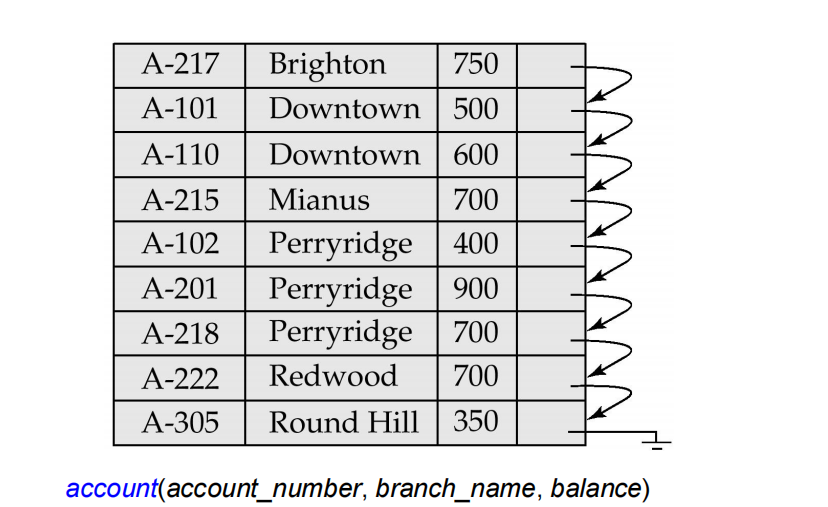
\includegraphics[width=0.8\linewidth]{image2.png}
    \caption{例}
    \label{}
\end{figure}

假设:账户按照搜索键分行名称进行排序。
\texttt{Select * from account where branch\_name = 'Downtown';}
可能会返回100个元组。

\subsection{使用索引和相等条件进行选择}

索引扫描---使用索引的搜索算法:选择条件必须基于索引的搜索键。

\noindent算法A3(主索引,键上的相等条件),检索满足相应相等条件的单条记录。成本$=(h_i+1)*(t_S+t_T)$,其中$h_i$为索引树高。

\noindent算法A4(主索引,非键上的相等条件)检索多条记录。记录将位于连续的块上,设$b=$为包含匹配记录的块数,成本$=h_i*(t_S+t_T)+t_S+t_T*b$

\noindent算法A5(二级索引,非键上的相等条件)
\begin{itemize}
    \item 如果搜索键是候选键,则检索单条记录:成本$=(h_i+1)*(t_T+t_S)$
    \item 如果搜索键不是候选键,则检索多条记录。每个$n$匹配记录可能位于不同的块上,成本$=(h_i+n)*(t_T+t_S)$,可能代价非常高,可能比线性扫描更糟糕。
\end{itemize}

\subsection{涉及比较的选择}

比较符:$>,\geq,<.\leq,<>$,与等值比较不同之处在于选择范围大。

可以通过以下方式实现$\sigma_{A\leq V}(r)$或$\sigma_{A\geq V}(r)$形式的选择:
\begin{itemize}
    \item[a] 线性文件扫描;
    \item[b] 二分查找(如A2);
    \item[c] 以下方式使用索引:
\end{itemize}

\noindent算法A6(基于主索引的比较):
\begin{itemize}
    \item 对于$\sigma_{A\geq V}(r)$,使用索引查找第一个元组$A\geq v$并从那里开始顺序扫描关系
    \item 对于$\sigma_{A\leq V}(r)$,只需顺序扫描关系直到找到第一个元组$A\geq v$;不使用索引
\end{itemize}

\noindent算法A7(基于辅助索引的比较)
\begin{itemize}
    \item 对于$\sigma_{A\geq V}(r)$,使用索引查找第一个索引项$\geq v$并从那里开始顺序扫描索引,以找到指向记录的指针。
    \item 对于$\sigma_{A\leq V}(r)$,只需扫描索引的叶页以查找指向记录的指针,直到遇到第一个目录$A>v$
    \item 在这两种情况下,检索所指向的记录:每条记录都需要一个I/O;线性文件扫描可能成本更低。
\end{itemize}

\subsection{复杂选择的实现}

合取:$\sigma_{\theta_1}\land \sigma_{\theta_2}\land ...\sigma_{\theta_n}(r)$

\noindent算法A8(使用一个索引进行合取选择):
\begin{itemize}
    \item 选择$\theta_l$的组合,以及算法A1到A7,使得$\theta_l$的代价最小(第一步从$n$个条件$\theta_1...\theta_n$中选择代价最小的$\theta_i$先执行,返回元组放内存,然后第二步对这些元组施行其它$\theta_j$)
    \item 将元组提取到内存缓冲区后,对其进行其它条件测试。
\end{itemize}

\noindent算法A9(使用复合索引进行连接选择):若可用,使用适当的复合(多键)索引。

\noindent算法10(通过标识符交集进行连接选择):
\begin{itemize}
    \item 需要带有记录指针的索引。
    \item 为每个条件使用相应的索引,并取所有的交集获取的记录指针集。
    \item 然后从文件中提取记录
    \item 如果某些条件没有合适的索引,则在内存中进行测试。
\end{itemize}

析取:$\sigma_{\theta_1}\lor \sigma_{\theta_2}\lor...\sigma_{\theta_n}(r)$

\noindent算法10(通过标识符的并集进行析取选择)
\begin{itemize}
    \item 如果所有条件都有可用索引,则适用。否则使用线性扫描。
    \item 为每个条件使用相应的索引,并取所有获得的记录指针集合的并集。
    \item 然后从文件中提取记录。
\end{itemize}

否定:$\sigma_{\lnot \theta}(r)$
\begin{itemize}
    \item 对文件使用线性扫描
    \item 如果只有极少数记录满足$\lnot \theta$,并且索引适用于$\theta-$使用索引查找满足条件的记录并从文件中提取
\end{itemize}